

\subsection{Designing a Basic CAN Network}
\label{sub:TestingCANStack_BareMetal}
This section includes the design and development of hardware and software in order to realize the CAN network.
This software and hardware co-design was developed firstly to establish a basic CAN network between a number of Zybo boards and secondly to prove and test the functionality of the CAN stack designed for this project.
It was also meant to be the basis for the development of the CAN controller part of the full system but in the end it was only used for testing purposes, as described in section \ref{sub:CAN_Bus_Tests}.

\subsubsection{Hardware Architecture}
The initial design of the hardware included enabling the CAN controller inside the Zynq chip as well as the addition of two AXI GPIO cores.
One AXI GPIO was setup as leds 4bits while the other one as btns 4bits as it can be seen in figure \ref{fig:CAN_Testing_Architecture}.
The architecture was firmly simple, but adequate to meet the purpose of basic communication between nodes.
Later on the design was updated with one more AXI GPIO core that was added to provide interrupts on an external GPIO port.

\begin{figure}[h!]
	\centering
	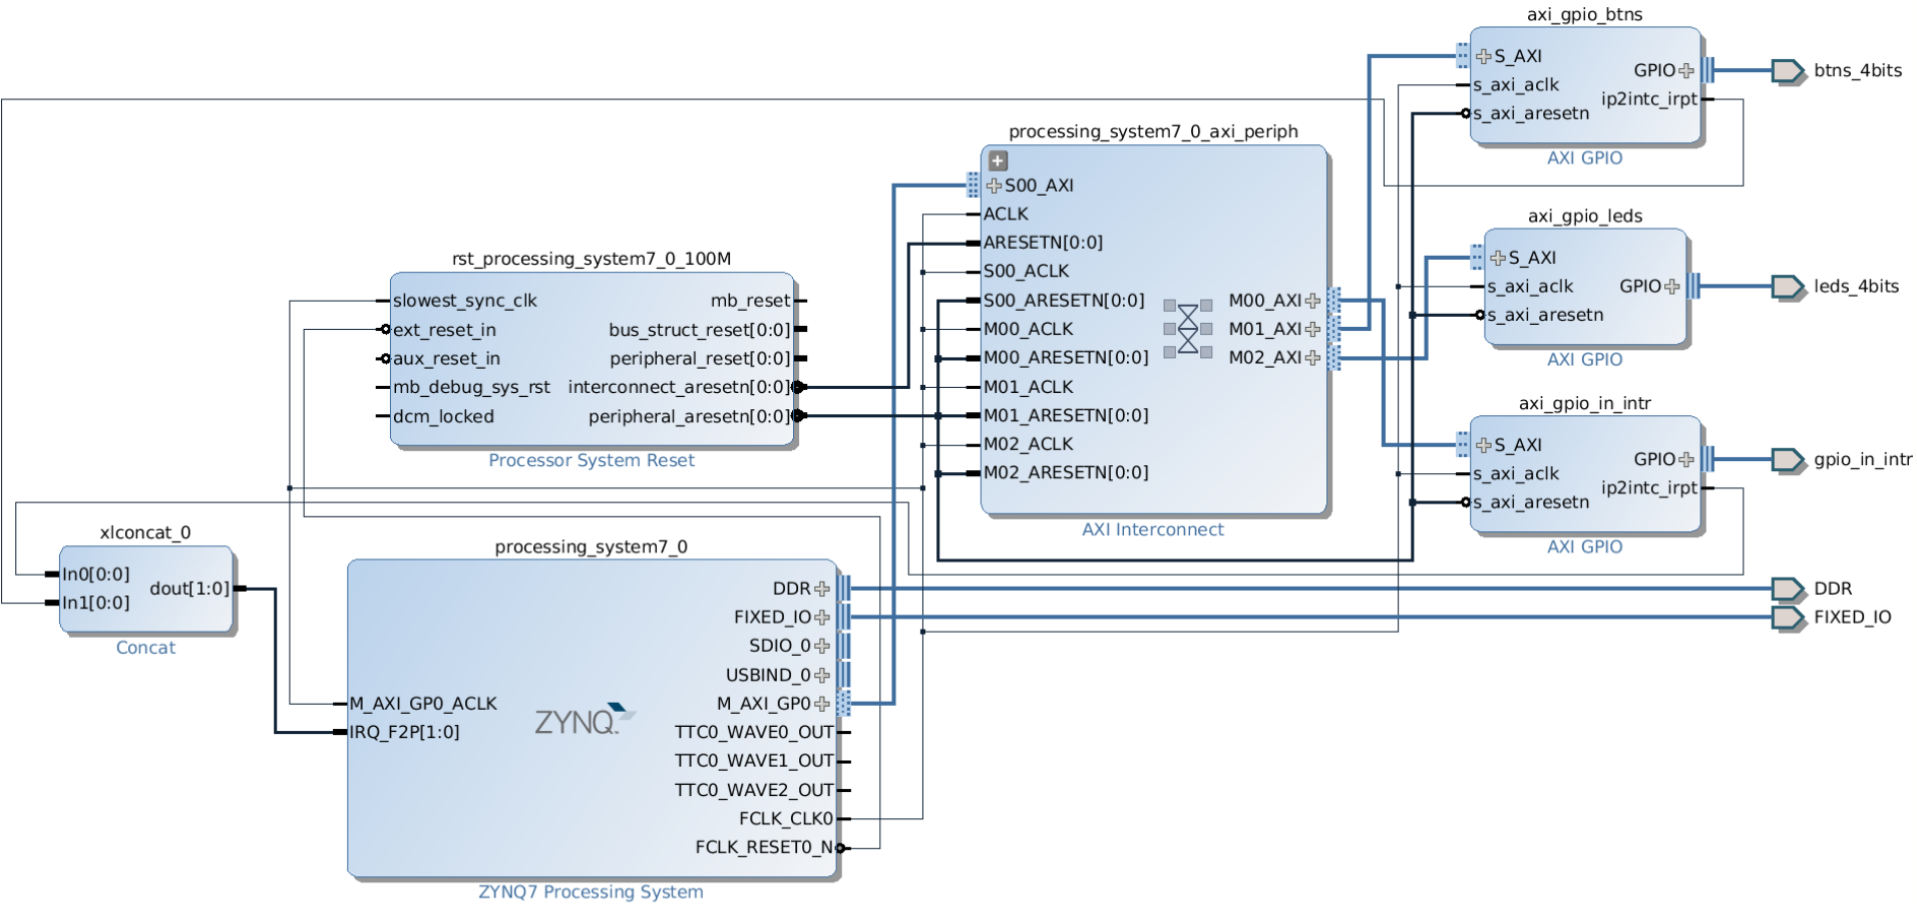
\includegraphics[width = 1.1\linewidth]{graphics/Zybo_BasicTestingArchitecture_for_CAN.png}
	\caption{Block diagram featuring the architecture in Vivado.}
	\label{fig:CAN_Testing_Architecture}
\end{figure}
\catalin{Alternative word to non-final version}
\catalin{Bullet list: 1st letters capitals or not?}
\subsubsection{Software Functionalities}~\\
\label{sub:Basic_SourceCode}
The programming for this task was done in C.
The code from xcanps polled example provided by Xilinx was used as a basis.
The example shows the basic principle of sending and receiving messages on a CAN network in the Processing System on a single board.
With further modifications and the addition of extra functionalities such as reading button input and writing the output to the LEDs, the finalized developed code was suitable to test the communication between two nodes on the CAN network, as described in section \ref{sub:TestingCANStack_BareMetal}.
The basic principle for proving the basic communication was to trigger an interrupt attached to the button presses, which then the SendFrame() function would send the value of the buttons to the network as a message.
In turn, the RecvFrame() was responsible of reading the message transmitted on the bus and writing the value as output to the LEDs.
The important functionalities that needed to be provided by the non-final version of this software included:
\begin{itemize}
\item receiving and sending of frames
\item creating the message id
\item decoding of the message id parts, such as the node id, the message type and the command
\item handling interrupts from buttons and a GPIO port
\item controlling the LEDs
\item accepting and ignoring messages according to a subscriptions list
\end{itemize}

\subsubsection{Publisher-Subscriber Architecture}
\catalin{Should I explain more about the architecture? Or is it the readers responsibility to read about it?}
A mechanism was also necessary to control the receivers and transmitters of messages.
One of the functionalities of the network was to provide the ability for various nodes to be able to send specific messages to other nodes.
Such a mechanism could easily be implemented using the Publisher-Subscriber architecture which would also make the network data-driven.
Using this method, the communication among the various nodes could be easily configured just by adding messages ids to an array variable containing the node's subscriptions.
The use of this architecture was incorporated in the protocol functionality, along with a set of functions in the source code and an array variable of subscriptions for each node.

\subsubsection{Main Loop}
Since the whole system, that was intended to be designed for this project, could not be put together, an approach to simulate the network in various ways was needed.
Specifically, sending arbitrary messages was achieved by implementing button interrupts
\catalin{Talk and decide on the matter of GPIO interrupts.}
%\martin{I removed some text, that doesn't fit with the validation part}
%and the case where multiple nodes would send messages simultaneously by GPIO port interrupts.
%For details on how the different tests were done the reader may refer to section \ref{sub:CAN_Bus_Tests}.
%Due to conflicts between the interrupt controllers and handlers, only one of the two simulation cases could be active during runtime.
%Depending on the value of a macro definition in the source code the desired devices (buttons or GPIO) would be initialized.

\paragraph{Runtime with Button Interrupts}~\\
During execution, the program runs permanently in a while loop waiting for receiving data in the FIFO.
When data arrives, the LEDs are controlled using the values contained in the RxFrame, as seen in figure \ref{fig:FlowChart_CANSoft_RecvData}.
An interrupt handler is also enabled, which when a button is being pressed, it reads the buttons input and send a CAN message containing their value as data. The process of sending a TxFrame is shown in the flow chart in figure \ref{fig:FlowChart_CANSoft_BtnsIntr}.

\begin{figure}[h!]
	\centering
	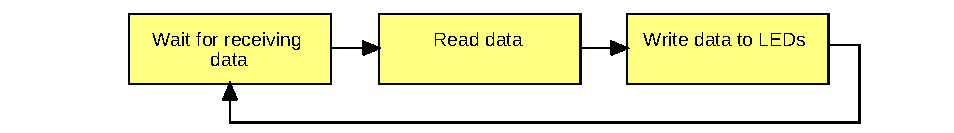
\includegraphics[width = 1\linewidth]{graphics/FlowChart_CANSoft_RecvData.pdf}
	\caption{Flow chart for the process of receiving data.}
	\label{fig:FlowChart_CANSoft_RecvData}
\end{figure}
\begin{figure}[h!]
	\centering
	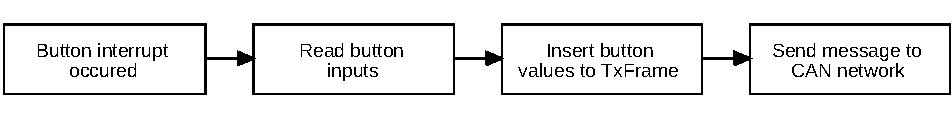
\includegraphics[width = 1\linewidth]{graphics/FlowChart_CANSoft_BtnsIntr.pdf}
	\caption{Flow chart with button interrupts.}
	\label{fig:FlowChart_CANSoft_BtnsIntr}
\end{figure}

\paragraph{Runtime with GPIO Interrupts}~\\
\martin{Do we use this? I didn't use interrupts for my code}
The software's behavior is similar in this case, as well as it can be seen in figure \ref{fig:FlowChart_CANSoft_GPIOIntr}.
The difference is that instead of button values, dummy data may be inserted into the TxFrame according to the simulation needs and the receiving data is only presented in the SDK terminal.
\begin{figure}[h!]
	\centering
	
\includegraphics[width = 1\linewidth]{graphics/FlowChart_CANSoft_GPIOIntr.pdf}
	\caption{Flow chart with GPIO interrupts.}
	\label{fig:FlowChart_CANSoft_GPIOIntr}
\end{figure}

\subsubsection{Sending and Receiving Frames}
\martin{Catalin: I explained createMsgID, is it good enough? Are you happy? Are you satisfied?}
The figure \ref{fig:SeqDiagram_SendFrame} shows the procedure of sending a frame to the CAN network containing data, which makes use of the protocol function createMsgID().
In the full implementation of the system the message id would be provided by the software running in the userspace but since this was not the case this function was necessary.
Its purpose is to put together the priority bit, the sender id and the message type into the 11 bit message id.
After returning the message id, the id and the data are put into the TxFrame to be sent once the FIFO has space.
The actual sending is done with a call to the XCanPs function XCanPs\_Send().
\\
Similarly, the procedure of receiving a frame is shown in the figure \ref{fig:SeqDiagram_RecvFrame}.
The node once it calls the RecvFrame() function, it waits in a loop until it receives a frame.
Then, it checks the subscriptions in order to forward the packet for further processing or to ignore it.
In both cases appropriate messages using the function xil\_printf() are presented to the developer in the SDK terminal.

\begin{figure}[h!]
	\centering
	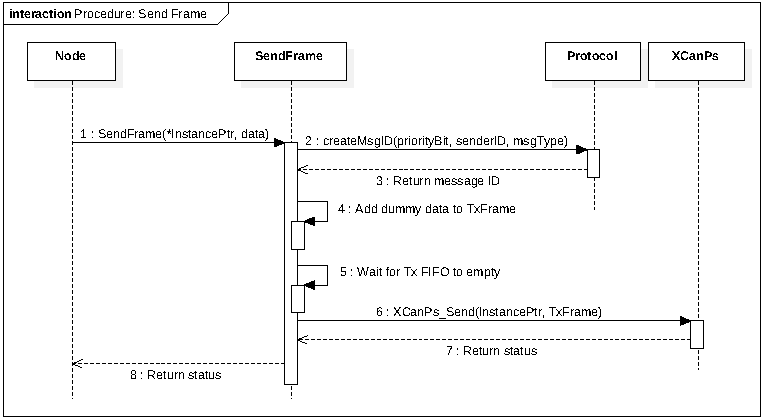
\includegraphics[width = 1\linewidth]{graphics/SeqDiagram_SendFrame.pdf}
	\caption{The sequence diagram of the process of sending a frame.}
	\label{fig:SeqDiagram_SendFrame}
\end{figure}

\begin{figure}[h!]
	\centering
	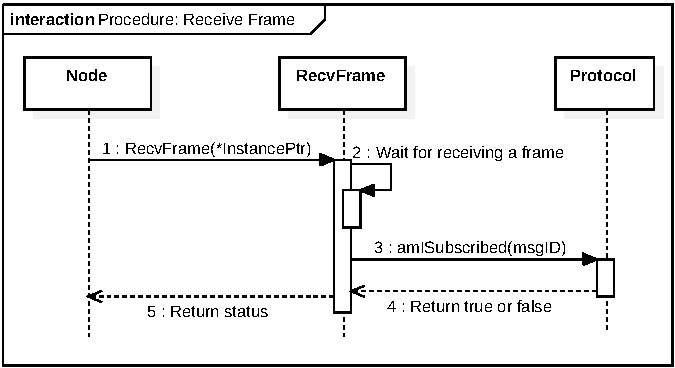
\includegraphics[width = 1\linewidth]{graphics/SeqDiagram_RecvFrame.pdf}
	\caption{The sequence diagram of the process of receiving a frame.}
	\label{fig:SeqDiagram_RecvFrame}
\end{figure}